%----------------------------------------------------------------------------
\chapter{Áttekintés}
\label{sec:overview}
%----------------------------------------------------------------------------
\section{A perifériaillesztő modul felépítése}
%----------------------------------------------------------------------------

% \begin{center}
%     \begin{tikzpicture}
%         \tikzset{
%             top/.style= {draw, rectangle, inner sep=20pt, minimum height=0.6\textwidth, minimum width=0.8\textwidth, align=center},
%             module/.style= {draw, rectangle, minimum height=0.5\textwidth ,minimum width=0.3\textwidth},
%             input/.style  = {coordinate},
%             output/.style = {coordinate}}
%         \node[input] (PCLK) at (-0.55\textwidth, 0.21875\textwidth) {};
%         \node[input] (PRESETn) at (-0.55\textwidth, 0.15625\textwidth) {};
%         \node[input] (PADDR) at (-0.55\textwidth, -0.09375\textwidth) {};
%         \node[input] (PSELx) at (-0.55\textwidth, 0.03125\textwidth) {};
%         \node[input] (PENABLE) at (-0.55\textwidth, -0.03125\textwidth) {};
%         \node[input] (PWRITE) at (-0.55\textwidth, -0.09375\textwidth) {};
%         \node[input] (PRDATA) at (-0.55\textwidth, -0.15625\textwidth) {};
%         \node[input] (PWDATA) at (-0.55\textwidth, -0.21875\textwidth) {};
%         \node[output] (SCL) at (0.55\textwidth, 0) {};
%         \node[module] (APB) at (-0.3\textwidth, 0) {};
%         \node[above left] at (APB.south east) {mod\_apb};
%         \draw[->] (PCLK) -- node[auto] {PCLK} (APB.west);
%         \draw[->] (PRESETn) -- node[auto] {PRESETn} (APB.west);
%         \draw[->] (PADDR) -- node[auto] {PADDR} (APB.west);
%         \draw[->] (PSELx) -- node[auto] {PSELx} (APB.west);
%         \draw[->] (PENABLE) -- node[auto] {PENABLE} (APB.west);
%         \draw[->] (PWRITE) -- node[auto] {PWRITE} (APB.west);
%         \draw[->] (PRDATA) -- node[auto] {PRDATA} (APB.west);
%         \node[module] (I2C) at (0.3\textwidth, 0) {};
%         \node[above left] at (I2C.south east) {mod\_i2c};
%         \draw[->] (I2C.east) -- node[auto] {SCL} (SCL);
%         \node[top, fit=(APB)(I2C)] (TOP) at (0,0) {};
%         \node[above left] at (TOP.south east) {mod\_top};
%         % \node[]
%     \end{tikzpicture}
% \end{center}
Mint az a \figref{modtop} ábrán is látszik, modulunk (\emph{mod\_top}) 2 almodult tartalmaz, a feladatkíírásnak megfelelően: egy \emph{mod\_apb} modulból, ami közvetlenül az APB buszra csatlakozik, és egy \emph{mod\_i2c} modulból, ami a soros kommunkáció vonalaival van összeköttetésben.

\begin{figure}[ht!]
    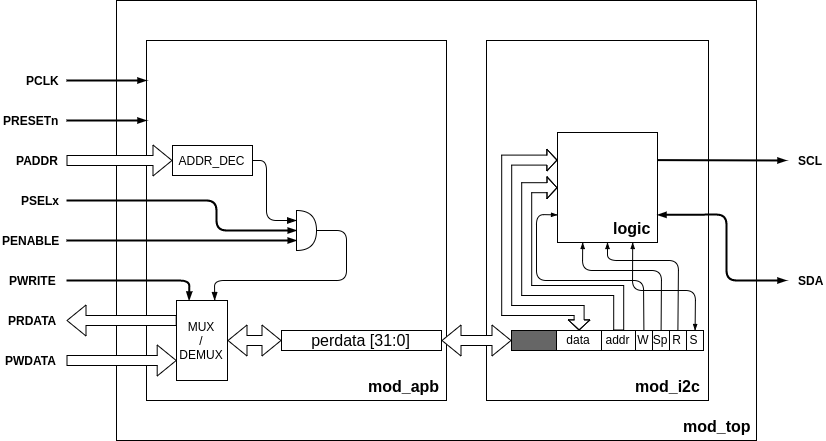
\includegraphics[width=\textwidth]{figures/overview}
    \caption{A modul magas szintű áttekintő ábrája.}
    \label{fig:modtop}
\end{figure}

Az APB modul a rendszerbusz vezérlőjeleit dekódolja, és továbbítja a szükséges adatokat az I2C modulnak.
Az I2C modul a rendelkezésére bocsátott adatokból lefolytatja soros kommunikációt.

A továbbiakban tekintsük át részletesebben az almodulok felépítését.

\section{mod\_apb}
\section{mod\_i2c}
